\documentclass[headinclude,DIV12]{scrartcl}

\usepackage[latin1]{inputenc}
\usepackage[T1]{fontenc}
\usepackage[english]{babel}

\usepackage{scrpage2}
\usepackage{url}
%
\usepackage{pst-optexp}
\let\verPstOptExp\fileversion
\let\datePstOptExp\filedate
\usepackage{multicol}
\usepackage{showexpl}
\lstset{breakatwhitespace}
\usepackage{nicefrac}
\usepackage{graphicx}
\usepackage[colorlinks,linktocpage]{hyperref}
%
% New commands
%
\DeclareRobustCommand\cs[1]{\texttt{\char`\\#1}}
\newcommand{\OptExpPackage}{\textsf{`pst-optexp'}}
\newcommand{\parameter}[1]{\texttt{#1}}
\let\param\textrm
\newcommand{\paramvalue}[1]{\texttt{#1}}
\newcommand{\defaultparam}[1]{\emph{default:} \paramvalue{#1}}
\def\lbracket{[}
\def\rbracket{]}

%
% Settings
\setkomafont{sectioning}{\normalfont\normalcolor\bfseries}
%
\makeatletter
\renewenvironment{description}
  {\list{}{\labelwidth\z@ \itemindent-\leftmargin
    \itemsep0pt \parsep0pt
    \let\makelabel\descriptionlabel}}
  {\endlist}
\makeatother
%
\clearscrheadfoot
\setheadsepline{0.4pt}
\ihead{\OptExpPackage}\ohead{A PSTricks package to draw optical experimental setups}
\ofoot{\pagemark}
\pagestyle{scrheadings}

\psset{subgriddiv=0,griddots=10,gridlabels=7pt}

%%%%%%%%%%%%%%%%%%%%%%%%%%%%%%%%%%%%%%%%%%%%%%%%%%%%%%%%%%%%%%%%%%%%%%%%
\begin{document}
 \title{\texttt{pst-optexp}\\ A PSTricks package to draw optical experimental setups}
 \author{Christoph Bersch \textless
   \href{mailto:usenet@bersch.net}{\texttt{usenet@bersch.net}}\textgreater}
 \date{\datePstOptExp\enspace\enspace Version \verPstOptExp}

\maketitle

\setlength{\columnseprule}{0.6pt}
\begin{multicols}{2}
{\parskip 0pt \tableofcontents}
\end{multicols}
\section{Introduction}
The package \texttt{pst-optexp} is a collection of optical components
that facilitate easy sketching of optical experimental
setups. Mechanisms for proper alignment of different components are
provided internally. This way the user does not have to care for proper
orientation of the elements. Macros for convenient definition of new 
user-defined components are also provided.

\section{Components}

In the sections \ref{sec:lens}--\ref{sec:custom} the
available components with their parameters are described. Up to now
there are two types of components: those which require two reference
points and do not alter the direction of the passing light beam (for
example lenses and retardation plates) and those which work in
reflection and require three reference points (mirrors, grids,
beamsplitters etc.).

In section \ref{sec:general} general parameters are described that are
not proprietary to a specific unit but can be used for several different
components. Finally, in section \ref{sec:labels} the options for the
positioning of labels are explained.

The appearence of all components can be changed with the corresponding
standard PSTricks parameters such as \parameter{fillstyle}
or \parameter{linestyle}. For some components changing only parts of the
layout is possible (e.g. the extended part of mirrors). For those cases
psstyles are provided that influence only the corresponing part of the
components and can be redefined using \cs{newpsstyle}.

\subsection{Free-ray components}

\subsubsection{Lens}\label{sec:lens}

\begin{description}
\item[\param{lensheight}:] \paramvalue{<value>} (\defaultparam{1})
\item[\param{lenswidth}:] \paramvalue{<value>} (\defaultparam{0.3})
\item[\param{lensradius}:] \paramvalue{<value> [<value>]} (\defaultparam{\cs{empty}})
\item[\param{lensradiusleft}:] \paramvalue{<value>} (\defaultparam{1})
\item[\param{lensradiusright}:] \paramvalue{<value>} (\defaultparam{1})
\item[\param{lens}:] \paramvalue{<value> [<value> [<value> [<value>]]]} (\defaultparam{\cs{empty}})
\item[\param{thicklens}:] \paramvalue{<boolean>}(\defaultparam{false})
\end{description}

\medskip 

\begin{LTXexample}[width=5.5cm]
\begin{pspicture}(5,6)\psgrid
  % concave lenses
  \pnode(0,5){A}\pnode(5,5){B}
  \psline[style=OptBeam](A)(B)
  \lens[position=0.2](A)(B){L}
  \lens[lensradius=-1,position=0.5](A)(B){L}
  \lens[lens=-1.5 1,position=0.7](A)(B){L}
  % convex lenses
  \pnode(0,3){A}\pnode(5,3){B}
  \psline[style=OptBeam](A)(B)
  \lens[position=0.2,lens=1 -1](A)(B){L}
  \lens[lens=0 -1](A)(B){L}
  \lens[lens=1 0,position=0.7](A)(B){L}
  % thick lenses
  \pnode(0,1){A}\pnode(5,1){B}
  \psline[style=OptBeam](A)(B)
  \lens[position=0.3,lens=-1.5 1 1 0.5,thicklens](A)(B){thicklens}
  \lens[lens=0 -1, position=0.7, fillstyle=solid, fillcolor=blue!30!white](A)(B){lens}
\end{pspicture}
\end{LTXexample}

\medskip

The shape of a lens is defined by its two surface radii. A negative
radius gives a concave, a positive radius a convex and a radius of
\texttt{0} a plain surface. The parameters \parameter{lensradiusleft}
and \parameter{lensradiusright} allow to define independent values for both
surfaces. \parameter{lensradius} sets both curvatures to the same
value. Usually only \parameter{lensheight} and the two radii are used to
construct the lens. The thickness (or width) is determined
automatically. Manually controlling the thickness of the lens can be
achived by setting \parameter{thicklens}
to \parameter{true}. Then \parameter{lenswidth} is used as width of the lens at
its waist. Finally, the parameter \parameter{lens} allows the definition of
all relevant lens parameters at once. It consists of one up to four
space-separated numbers. The first one gives the left radius. If no
further value is set, the right radius will be set to the same value and
all other parameters are left unchanged. Using two numbers defines two
different radii. The third optional value defines
the \parameter{lensheight} and the fourth one the \parameter{lenswidth}

\textbf{Compatibility:} The whole implementation of the lens was
changed in version 1.2. It allows a much more flexible definition of different lens
types. However, I could not get full compatibility with the older way to
define lens using only \parameter{lensheight} and \parameter{lenswidth}. To use
this old behaviour, you have to set the \parameter{lenstype} explicitly, but
then you have no access to the new features! All users are encouraged to
adapt their code to use the new parameters, as the old code will be
removed in future versions.

\medskip
\subsubsection{Optical plate}

\begin{description}
\item[\param{plateheight}:] \paramvalue{<value>} (\defaultparam{1})
\item[\param{platelinewidth}:] \paramvalue{<value>} (\defaultparam{2\cs{pslinewidth}})
\end{description}

\medskip

\begin{LTXexample}[width=3.5cm]
\begin{pspicture}(3,2)\psgrid
  \pnode(0,1.2){A}
  \pnode(3,1.2){B}
  \psline[style=OptBeam](A)(B)
  \optplate(A)(B){filter}
\end{pspicture}
\end{LTXexample}

\medskip

\subsubsection{Retardation plate}

\begin{description}
\item[\param{plateheight}:] \paramvalue{<value>} (\defaultparam{1})
\item[\param{platewidth}:] \paramvalue{<value>} (\defaultparam{0.1})
\end{description}

\medskip

\begin{LTXexample}[width=3.5cm]
\begin{pspicture}(3,2)\psgrid
  \pnode(0,1.2){A}
  \pnode(3,1.2){B}
  \psline[style=OptBeam](A)(B)
  \optretplate(A)(B){$\nicefrac{\lambda}{2}$}
\end{pspicture}
\end{LTXexample}

\medskip

\subsubsection{Pinhole}

\begin{description}
\item[\param{outerheight}:] \paramvalue{<value>} (\defaultparam{1})
\item[\param{innerheight}:] \paramvalue{<value>} (\defaultparam{0.1})
\item[\param{phlinewidth}:]  \paramvalue{<value>} (\defaultparam{2\cs{pslinewidth}})
\end{description}

\medskip

\begin{LTXexample}[width=3.5cm]
\begin{pspicture}(3,2)\psgrid
  \pnode(0,1.2){A}
  \pnode(3,1.2){B}
  \psline[style=OptBeam](A)(B)
  \pinhole(A)(B){PH}
\end{pspicture}
\end{LTXexample}

\medskip

\subsubsection{Crystal}\label{sec:crystal}

\begin{description}
\item[\param{crystalwidth}:] \paramvalue{<value>} (\defaultparam{2})
\item[\param{crystalheight}:] \paramvalue{<value>} (\defaultparam{0.8})
\item[\param{caxislength}:] \paramvalue{<value>} (\defaultparam{0.6})
\item[\param{caxisinv}:] \paramvalue{<boolean>} (\defaultparam{false})
\item[\param{voltage}:] \paramvalue{<boolean>} (\defaultparam{false})
\item[\param{lamp}:] \paramvalue{<boolean>} (\defaultparam{false})
\item[\param{lampscale}:] \paramvalue{<value>} (\defaultparam{0.3})
\end{description}

\medskip

\begin{LTXexample}[width=3.5cm]
\begin{pspicture}(3,2)\psgrid
  \pnode(0,1.2){A}
  \pnode(3,1.2){B}
  \crystal[crystalwidth=1.5, crystalheight=0.6, fillstyle=solid, fillcolor=yellow!90!black, labelangle=-45, labeloffset=1.2, voltage, lamp](A)(B){SBN:Ce}
  \psline[style=OptBeam](A)(B)
\end{pspicture}
\end{LTXexample}

\medskip

\subsubsection{Box}

\begin{description}
\item[\param{optboxheight}:] \paramvalue{<value>} (\defaultparam{0.5})
\item[\param{optboxwidth}:] \paramvalue{<value>} (\defaultparam{1})
\item[\param{endbox}:] \paramvalue{<boolean>} (\defaultparam{false})
\end{description}

\medskip 

\begin{LTXexample}[width=3.5cm]
\begin{pspicture}(3,2)\psgrid
  \pnode(0,0){A}
  \pnode(3,2){B}
  \psline[style=OptBeam](A)(B)
  \optbox(A)(B){box}
\end{pspicture}
\end{LTXexample}

\bigskip

\begin{LTXexample}[width=3.5cm]
\begin{pspicture}(3,2)\psgrid
  \pnode(0,0){A}
  \pnode(1.7,1){B}
  \psline[style=OptBeam](A)(B)
  \optbox[endbox](A)(B){box}
\end{pspicture}
\end{LTXexample}

\bigskip

\begin{LTXexample}[width=3.5cm]
\begin{pspicture}(3,2)\psgrid
  \pnode(0,0){A}
  \pnode(1.7,1){B}
  \psline[style=OptBeam](A)(B)
  \optbox[endbox,labelref=relative,labeloffset=0](A)(B){box}
\end{pspicture}
\end{LTXexample}

\medskip

\subsubsection{Detector}

\begin{description}
\item[\param{detsize}:] \paramvalue{<value>} (\defaultparam{0.5})
\end{description}

\medskip 

\begin{LTXexample}[width=3.5cm]
\begin{pspicture}(3,2)\psgrid
  \pnode(0,0){A}
  \pnode(1.7,1){B}
  \psline[style=OptBeam](A)(B)
  \detector(A)(B){detector}
\end{pspicture}
\end{LTXexample}

\medskip

\subsubsection{Polarization}

\begin{description}
\item[\param{poltype}:] \paramvalue{parallel|perp|misc|lcirc|rcirc} (\defaultparam{parallel})
\item[\param{polsize}:] \paramvalue{<value>} (\defaultparam{0.6})
\item[\param{pollinewidth}:] \paramvalue{<value>} (\defaultparam{0.7\cs{pslinewidth}})
\end{description}

\medskip

\begin{LTXexample}[width=3.4cm]
\begin{pspicture}(3,5)\psgrid
  \pnode(0,0.5){A1}\pnode(3,0.5){B1}\pnode(0,1.5){A2}
  \pnode(3,1.5){B2}\pnode(0,2.5){A3}\pnode(3,2.5){B3}
  \pnode(0,3.5){A4}\pnode(3,3.5){B4}\pnode(0,4.5){A5}
  \pnode(3,4.5){B5}\psset{style=OptBeam}
  \multido{\i=1+1}{5}{\psline(A\i)(B\i)}
  \psset{linecolor=black}
  \polarization[poltype=misc,position=0.2](A5)(B5)
  \polarization[poltype=perp,position=0.35](A4)(B4)
  \polarization[poltype=parallel,position=0.5](A3)(B3)
  \polarization[poltype=rcirc,position=0.65](A2)(B2)
  \polarization[poltype=lcirc,position=0.8](A1)(B1)
\end{pspicture}
\end{LTXexample}

\medskip

\subsubsection{Mirror}\label{sec:mirror}

\begin{description}
\item[\param{mirrorwidth}:] \paramvalue{<value>} (\defaultparam{1})
\item[\param{mirrorradius}:] \paramvalue{<value>} (\defaultparam{0})
\item[\param{mirrorlinewidth}:] \paramvalue{<value>} (\defaultparam{2\cs{pslinewidth}})
\item[\param{mirrortype}:] \paramvalue{normal|piezo|extended} (\defaultparam{normal})
\item[\param{mirrordepth}:] \paramvalue{<value>} (\defaultparam{0.08})
\item[\param{variable}:] \paramvalue{<value>} (\defaultparam{false})
\end{description}

The parameter \texttt{mirrorradius} defines the curvature of the mirror. A
value of \texttt{0} is for a plain mirror, a negative radius is for a
concave mirror and a positive radius gives you a convex mirror. The
style of the extended mirror is defined as a
psstyle \parameter{ExtendedMirror} and can be changed using
\cs{newpsstyle}. The appearence of the piezo mirror likewise can be
changed by adapting the psstyle \parameter{PiezoMirror}.

\medskip

\begin{LTXexample}[width=3.5cm]
\begin{pspicture}(3,3)\psgrid
  \pnode(0,0){A}
  \pnode(1.8,2.2){G}
  \pnode(0,3){B}
  \psline[style=OptBeam](A)(G)(B)
  \mirror(A)(G)(B){mirror}
\end{pspicture}
\end{LTXexample}

\bigskip

\begin{LTXexample}[width=3.5cm]
\begin{pspicture}(3,3)\psgrid
  \pnode(0,0){A}
  \pnode(1.8,2.2){G}
  \pnode(0,3){B}
  \psline[style=OptBeam](A)(G)(B)
  \mirror[variable](A)(G)(B){M$_\mathrm{var}$}
\end{pspicture}
\end{LTXexample}

\bigskip

\begin{LTXexample}[width=3.5cm]
\begin{pspicture}(3,3)\psgrid
  \pnode(0,0){A}
  \pnode(1.8,2.2){G}
  \pnode(0,3){B}
  \psline[style=OptBeam](A)(G)(B)
  \mirror[mirrortype=piezo,labelangle=-90](A)(G)(B){piezo}
\end{pspicture}
\end{LTXexample}

\bigskip

\begin{LTXexample}[width=3.5cm]
\begin{pspicture}(3,3)\psgrid
  \pnode(0,0){A}
  \pnode(1.8,2.2){G}
  \pnode(0,3){B}
  \psline[style=OptBeam](A)(G)(B)
  \mirror[mirrortype=extended](A)(G)(B){M$_\mathrm{ext}$}
\end{pspicture}
\end{LTXexample}

\begin{LTXexample}[width=3.5cm]
\begin{pspicture}(3,3)\psgrid
  \pnode(0,0){A}\pnode(0.7,2){G1}
  \pnode(1.5,1){G2}\pnode(2,3){B}
  \psset{labeloffset=0.5}
  \psline[style=OptBeam](A)(G1)(G2)(B)
  \mirror[mirrortype=extended, mirrorradius=1](A)(G1)(G2){M$_v$}
  \mirror[mirrorradius=-1](G1)(G2)(B){M$_x$}
\end{pspicture}
\end{LTXexample}

\medskip

\subsubsection{Beamsplitter}

\begin{description}
\item[\param{bssize}:] \paramvalue{<value>} (\defaultparam{0.8})
\end{description}

\medskip

\begin{LTXexample}[width=3.5cm]
\begin{pspicture}(3,3)\psgrid
  \pnode(0,2){A}
  \pnode(2,2){G}
  \pnode(3,0){B}
  \psline[style=OptBeam](A)(G)(B)
  \beamsplitter(A)(G)(B){BS}
\end{pspicture}
\end{LTXexample}

\medskip


\subsubsection{Optical grid}

\begin{description}
\item[\param{optgridcount}:] \paramvalue{<integer>} (\defaultparam{10})
\item[\param{optgridwidth}:] \paramvalue{<value>} (\defaultparam{1})
\item[\param{optgridheight}:] \paramvalue{<value>} (\defaultparam{0.1})
\item[\param{optgriddepth}:] \paramvalue{<value>} (\defaultparam{0.05})
\item[\param{optgridtype}:] \paramvalue{blazed|binary} (\defaultparam{blazed})
\item[\param{optgridlinewidth}:] \paramvalue{<value>} (\defaultparam{0.7\cs{pslinewidth}})
\item[\param{reverse}:] \paramvalue{<boolean>} (\defaultparam{false})
\end{description}

\medskip

\begin{LTXexample}[width=3.5cm]
\begin{pspicture}(3,3)\psgrid
  \pnode(0,3){A}
  \pnode(1.8,2.2){G}
  \pnode(0,0){B}
  \psline[style=OptBeam](A)(G)(B)
  \optgrid(A)(G)(B){grid}
\end{pspicture}
\end{LTXexample}

\bigskip


\begin{LTXexample}[width=3.5cm]
\begin{pspicture}(3,3)\psgrid
  \pnode(0,3){A}
  \pnode(1.8,2.2){G}
  \pnode(0,0){B}
  \psline[style=OptBeam](A)(G)(B)
  \optgrid[reverse](A)(G)(B){grid}
\end{pspicture}
\end{LTXexample}

\bigskip

\begin{LTXexample}[width=3.5cm]
\begin{pspicture}(3,3)\psgrid
  \pnode(0,3){A}
  \pnode(1.8,2.2){G}
  \pnode(0,0){B}
  \psline[style=OptBeam](A)(G)(B)
  \optgrid[optgridcount=6,%
           optgriddepth=0.2,%
           optgridheight=0.3](A)(G)(B){grid}
\end{pspicture}
\end{LTXexample}

\bigskip

\begin{LTXexample}[width=3.5cm]
\begin{pspicture}(3,3)\psgrid
  \pnode(0,3){A}
  \pnode(1.8,2.2){G}
  \pnode(0,0){B}
  \psline[style=OptBeam](A)(G)(B)
  \optgrid[optgridtype=binary](A)(G)(B){grid}
\end{pspicture}
\end{LTXexample}

\medskip

\subsubsection{Custom components}\label{sec:custom}
The macros \cs{optdipole} and \cs{opttripole} allow using everything as
optical component. If you want to use a certain component several times,
you should define it as a new component. For details see
sec.~\ref{sec:newobj}.

\begin{LTXexample}[width=3.5cm]
\begin{pspicture}(3,3)\psgrid
  \pnode(0,2){A}
  \pnode(3,1){B}
  \optdipole[labeloffset=1](A)(B){%
    \rput(0,0){%
      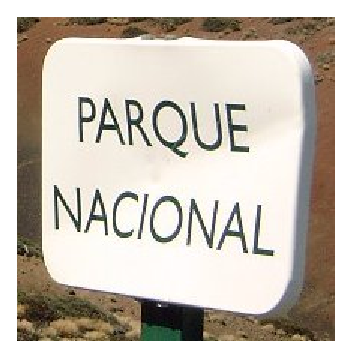
\includegraphics[scale=0.25]{parque-nacional}
    }
  }{label}
  \psline[linecolor=red](A)(B)
\end{pspicture}
\end{LTXexample}

\bigskip

\begin{LTXexample}[width=3.5cm]
\begin{pspicture}(3,3)\psgrid
  \pnode(0,0){A}
  \pnode(1.5,2){G}
  \pnode(3,1.5){B}
  \opttripole(B)(G)(A){\rput[b](0,0){text}}{label}
  \psline[linecolor=red](A)(G)(B)
\end{pspicture}
\end{LTXexample}

\medskip

\subsubsection{General options}\label{sec:general}

\begin{description}
\item[\param{angle}:] \paramvalue{<value>} (\defaultparam{0})
\item[\param{optional}:] \paramvalue{<boolean>} (\defaultparam{false})
\item[\param{position}:] \paramvalue{<value>} (\defaultparam{\cs{empty}})
\item[\param{abspos}:] \paramvalue{<value>} (\defaultparam{\cs{empty}})
\item[\param{showoptdots}:] \paramvalue{<boolean>} (\defaultparam{false})
\end{description}

The parameter \parameter{angle} is available for the macros \cs{optbox}
and \cs{crystal} only, as for the most other cases it would make
no sense. \parameter{optional} can be used with every component and marks it as
optional and can be configured by changing the psstyle \parameter{OptionalStyle}.
\parameter{position} is equivalent to the \parameter{npos} parameter of \cs{ncput},
but is used only for the \lq dipole\rq-macros to position the component
between the two given points. In addition, there is a parameter
\parameter{abspos} that allows absolute positioning between the two line
points. \parameter{showoptdots} shows in black the two points calculated for the
positioning of the component, and in red the reference points for the
label.

\medskip

\begin{LTXexample}[width=3.5cm]
\begin{pspicture}(3,2)\psgrid
  \pnode(0,1.2){A}
  \pnode(3,1.2){B}
  \psline[style=OptBeam](A)(B)
  \optbox[angle=10](A)(B){box}
\end{pspicture}
\end{LTXexample}

\bigskip

\begin{LTXexample}[width=3.5cm]
\begin{pspicture}(3,2)\psgrid 
  \pnode(0,1.2){A} 
  \pnode(3,1.2){B}
  \psline[style=OptBeam](A)(B) 
  \lens[optional](A)(B){L}
\end{pspicture}
\end{LTXexample}

\bigskip

\begin{LTXexample}[width=3.5cm]
\begin{pspicture}(3,2)\psgrid 
  \pnode(0,1.2){A} 
  \pnode(3,1.2){B}
  \psline[style=OptBeam](A)(B) 
  \lens[position=0.8](A)(B){L}
\end{pspicture}
\end{LTXexample}

\bigskip

\begin{LTXexample}[width=3.5cm]
\begin{pspicture}(3,2)\psgrid 
  \pnode(0,1.2){A} 
  \pnode(3,1.2){B}
  \psline[style=OptBeam](A)(B) 
  \lens[abspos=1](A)(B){L}
\end{pspicture}
\end{LTXexample}

\bigskip

\begin{LTXexample}[width=3.5cm]
\begin{pspicture}(3,3)\psgrid 
  \pnode(0,0){A} 
  \pnode(1.5,2){G}
  \pnode(0,3){B} 
  \psline[style=OptBeam](A)(G)(B)
  \mirror[showoptdots](A)(G)(B){mirror}
\end{pspicture}
\end{LTXexample}

\medskip

\subsection{Fiber-optical components}

\subsubsection{Fiber}
\begin{description}
\item[\param{fiberloops}:] \paramvalue{<integer>} (\defaultparam{3})
\item[\param{fiberloopradius}:] \paramvalue{<value>} (\defaultparam{0.3})
\item[\param{fiberloopsep}:] \paramvalue{<value>} (\defaultparam{0.3})
\end{description}
\medskip

\begin{LTXexample}[width=3.5cm]
\begin{pspicture}(3,2)\psgrid
  \optfiber(0,1)(3,1){SSMF}
\end{pspicture}
\end{LTXexample}

\medskip

\subsubsection{Amplifier}
\begin{description}
\item[\param{optampsize}:] \paramvalue{<value>} (\defaultparam{0.8})
\end{description}

\medskip

\begin{LTXexample}[width=3.5cm]
\begin{pspicture}(3,2)\psgrid
  \optamp(0,1)(3,1){EDFA}
\end{pspicture}
\end{LTXexample}

\medskip

\subsubsection{Mach-Zehnder Modulator}
\begin{description}
\item[\param{optmzmsize}:] \paramvalue{<value>} (\defaultparam{0.8})
\end{description}

\medskip

\begin{LTXexample}[width=3.5cm]
\begin{pspicture}(3,2)\psgrid
  \optmzm(0,1)(3,1){MZM}
\end{pspicture}
\end{LTXexample}

\medskip

\subsubsection{Filter}
\begin{description}
\item[\param{filtertype}:] \paramvalue{bandpass|bandstop} (\defaultparam{bandpass})
\end{description}

\medskip

\begin{LTXexample}[width=3.5cm]
\begin{pspicture}(3,2)\psgrid
  \optfilter(0,1)(3,1){bandpass}
\end{pspicture}
\end{LTXexample}

\bigskip

\begin{LTXexample}[width=3.5cm]
\begin{pspicture}(3,2)\psgrid
  \optfilter[filtertype=bandstop](0,1)(3,1){bandstop}
\end{pspicture}
\end{LTXexample}

\medskip

\subsubsection{Polarization controller}
\begin{description}
\item[\param{polcontrolsize}:] \paramvalue{<value>} (\defaultparam{0.1})
\end{description}

\medskip

\begin{LTXexample}[width=3.5cm]
\begin{pspicture}(3,2)\psgrid
  \polcontrol(0,1)(3,1){PC}
\end{pspicture}
\end{LTXexample}

\medskip

\subsubsection[2x2 Coupler]{$2\times 2$ Coupler}
\begin{description}
\item[\param{couplersize}:] \paramvalue{<value>} (\defaultparam{0.1})
\item[\param{couplerstyle}:] \paramvalue{free|elliptic} (\defaultparam{elliptic})
\end{description}

\medskip

\begin{LTXexample}[width=3.5cm]
\begin{pspicture}(3,2)\psgrid
  \optcoupler(0.5,2)(0,0.5)(3,1.5)(2.5,0){Coupler}
\end{pspicture}
\end{LTXexample}

\medskip

\subsection{Labels}\label{sec:labels}

\begin{description}
\item[\param{labeloffset}:] \paramvalue{<value>} (\defaultparam{1})
\item[\param{labelangle}:] \paramvalue{<value>} (\defaultparam{0})
\item[\param{labelstyle}:] \paramvalue{<macro>} (\defaultparam{\cs{small}})
\item[\param{labelalign}:] \paramvalue{<\cs{rput} ref string>} (\defaultparam{c})
\item[\param{labelref}:] \paramvalue{relative|relgrav|global} (\defaultparam{relgrav})
\end{description}

\parameter{labeloffset} specifies the offset from the center of the component, 
\parameter{labelstyle} defines the textstyle that is used to typeset the
label and \parameter{labelalign} corresponds to the refpoint of
\cs{rput}. The parameter \parameter{labelref} sets the reference
coordinate system for the \parameter{labelangle} and the orientation of
the label text. The detailed behaviour is best illustrated looking at
the following three examples.

\medskip

\begin{LTXexample}[width=5cm]
\begin{pspicture}(-2,-2)(2.5,2)
   \multido{\i=0+72}{5}{%
      \optbox[endbox,
              labelref=relative,
              labeloffset=0,
              optboxwidth=1](0,0)(1;\i){\i}
   }
\end{pspicture}
\end{LTXexample}

\bigskip

\begin{LTXexample}[width=5cm]
\begin{pspicture}(-2,-2)(2.5,2)
   \multido{\i=0+72}{5}{%
      \optbox[endbox,
              labelref=relgrav,
              optboxwidth=1](0,0)(1;\i){\i}
   }
\end{pspicture}
\end{LTXexample}

\bigskip

\begin{LTXexample}[width=5cm]
\begin{pspicture}(-2,-2)(2.5,2)
   \multido{\i=0+72}{5}{%
      \optbox[endbox,
              labelref=global,
              optboxwidth=1](0,0)(1;\i){\i}
   }
\end{pspicture}
\end{LTXexample}

\section{Defining new components}

\subsection{Customized versions of existing macros}

The easiest way to define your own components is to use the
\cs{newpsobject} macro. With this you can define a new component using
predefined objects with a set of options. These options serve only as
default values and can be overridden. The following examples defines a
new object \cs{sbn} for the special crystal used in
Sec.~\ref{sec:crystal}.

\medskip

\begin{LTXexample}[width=3.5cm]
\newpsobject{sbn}{crystal}{crystalwidth=1.5, crystalheight=0.6, voltage, lamp, labelangle=45, labeloffset=1.2, fillstyle=solid, fillcolor=yellow!90!black}
\begin{pspicture}(3,2)\psgrid 
   \sbn(0,1)(3,1){SBN:Ce}
   \psline[style=OptBeam](0,1)(3,1)
\end{pspicture}
\end{LTXexample}

\medskip

If you need more than one type of lenses in your setup it is very cumbersome to specify all parameters every time.

\medskip

\begin{LTXexample}[width=5.5cm]
\newpsobject{MOLensIn}{lens}{lens=0.5 0.5 0.5}
\newpsobject{MOLensOut}{lens}{lens=1.5 1.5 1.5}
\begin{pspicture}(5,2)\psgrid 
   \pnode(0,1){A}\pnode(5,1){B}
   \MOLensIn[abspos=0.5](A)(B){}
   \MOLensOut[abspos=1](A)(B){}
   \MOLensOut[abspos=4](A)(B){}
   \MOLensIn[abspos=4.5](A)(B){}
   \psline[style=OptBeam](A)(B)
\end{pspicture}
\end{LTXexample}
\medskip

\subsection{Defining new free-ray objects}\label{sec:newobj}

Since version 1.2 \texttt{pst-optexp} provides some high-level macros to
allow very convenient definition of completely new components. The macro
\cs{newOptexpDipole} generates all organizing code for the new
component. All you have to do is to define a new macro
\cs{mycomponent@iii} which contains all drawing code. Analogously
\cs{newOptexpDipoleNolabel} defines a new object which takes no label
(like \cs{polarization}) and \cs{newOptexpTripole} defines a new
reflective component.

The syntax of the macros is
\begin{lstlisting}
\newOptexpDipole[fixed options]{name}{default options}
\newOptexpDipoleNolabel[fixed options]{name}{default options}
\newOptexpTripole[fixed options]{name}{default options}
\end{lstlisting}
The \texttt{default options} are simply a list of PSTricks parameters which are taken as
defaults for the new component. The optional argument allows setting of parameters which 
cannot be overridden later.

This is illustrate a bit more in the next code snippet, which also shows
how the coordinate system is handled withing the \cs{mycomponent@iii}
macro.

\medskip

\begin{LTXexample}[width=4.5cm]
\newOptexpTripole{mygrid}{subgriddiv=5, griddots=0, subgridwidth=\pslinewidth, gridwidth=2\pslinewidth}
\makeatletter
\def\mygrid@iii{% put here all drawing code
  \psgrid(-1,0)(1,1)
}%
\makeatother
\begin{pspicture}(4,4)\psgrid 
   \pnode(0,1){A}\pnode(2,2){G}\pnode(3,0){B}
   \mygrid[gridcolor=red,labeloffset=1.5](A)(G)(B){myGrid}
   \psline[style=OptBeam](A)(G)(B)
\end{pspicture}
\end{LTXexample}
\medskip

The default position of the label reference point is (0,0). If you want
to change this, you have to define a new pnode named
\texttt{tempNode@Label} in the \cs{mycomponent@iii} macro.

If you create a new component, please send it to me then I can
incorporate this in a new released version.

\subsection{Defining new fiber objects}\label{sec:newfiberobj}
\newpage

\section{Examples}
\psset{unit=1.2cm}
\begin{LTXexample}[pos=t,vsep=8mm]
\begin{pspicture}(0,0.2)(12,1.8)
\pnode(0,1.2){Start}\pnode(11,1.2){CCD}
\psline[linewidth=2\pslinewidth,style=OptBeam](Start)(CCD)
\polarization[poltype=perp,position=0.1](Start)(CCD)
\optretplate[position=0.15](Start)(CCD){$\nicefrac{\lambda}{2}$}
\lens[lensheight=0.5,
      lensradius=0.5,
      position=0.25](Start)(CCD){$L_1$}
\lens[position=0.5](Start)(CCD){$L_2$}
\optplate[position=0.57, platelinewidth=3\pslinewidth](Start)(CCD){SLM}
\optplate[position=0.63](Start)(CCD){PF}
\polarization[position=0.66](Start)(CCD)
\lens[position=0.7](Start)(CCD){$L_3$}
\optbox[endbox,labeloffset=0](Start)(CCD){CCD}
\end{pspicture}
\end{LTXexample}

\vspace{\fill}

\begin{LTXexample}[pos=t,vsep=8mm]
\begin{pspicture}(-4,-1)(3,3)
  \psset{labeloffset=0.5}
  \pnode(-2,0){LaserOut}
  \pnode(0,0){Grid}
  \pnode(4;45){Out}
  \pnode(2.5;67.5){Mvar}
  \psline[linewidth=2\pslinewidth,
         linecolor=red!90!black](LaserOut)(Grid)(Out)\psline(Grid)(Mvar)
  \optbox[endbox, optboxwidth=2, labeloffset=0](Grid)(LaserOut){diodelaser}
  \optretplate[position=0.3, labeloffset=0.8](LaserOut)(Grid){$\nicefrac{\lambda}{4}$}
  \optgrid(LaserOut)(Grid)(Out){grid}
  \mirror[variable](Grid)(Mvar)(Grid){M$_\mathrm{var}$}
\end{pspicture}
\end{LTXexample}

\begin{LTXexample}[pos=t,vsep=3mm]
\begin{pspicture}(0,-0.4)(9,6)
  \pnode(1.5,5){Laser}\pnode(4,5){PBS}\pnode(6.5,5){PBS2}
  \pnode(6.5,5.7){piezo}\pnode(4,2){BSFwd}\pnode(6.5,2){BSBwd}
  \pnode(2,2){BS4f}\pnode(2,0.5){M4f3}\pnode(8,2){M4f1}
  \pnode(8,0.5){M4f2}\pnode(1,2){CCD}
  \psline[style=OptBeam,linewidth=2\pslinewidth]%
         (Laser)(PBS2)(piezo)(BSBwd)(M4f1)(M4f2)(M4f3)(BS4f)(CCD)
  \psline[style=OptBeam,linewidth=2\pslinewidth](PBS)(BSFwd)(BS4f)
  \psset{mirrorwidth=0.6, plateheight=0.7, outerheight=0.7, labeloffset=0.7, labelstyle=\scriptsize, lensheight=0.8, lenswidth=0.2, bssize=0.5} 
  \optbox[endbox,optboxwidth=1.5, optboxheight=0.7,labeloffset=0]%
     (PBS)(Laser){\parbox{1.5cm}{\centering Nd:YAG\\ 532\,nm}}
  \lens[lensheight=0.5, position=0.2](Laser)(PBS){MO}
  \pinhole[position=0.3,labelangle=180](Laser)(PBS){PH}
  \lens[position=0.5](Laser)(PBS){L}
  \optretplate[position=0.8](Laser)(PBS){$\nicefrac{\lambda}{2}$}
  \beamsplitter(Laser)(PBS)(BSFwd){PBS}
  \optretplate[position=0.4](PBS)(BSFwd){$\nicefrac{\lambda}{2}$}
  \polarization(PBS)(BSFwd)\polarization(PBS2)(BSBwd)
  \lens[position=0.8](PBS)(BSFwd){L}
  \optretplate(PBS)(PBS2){$\nicefrac{\lambda}{2}$}
  \beamsplitter(PBS)(PBS2)(piezo){PBS}
  \optretplate[abspos=0.5](PBS2)(piezo){$\nicefrac{\lambda}{4}$}
  \mirror[mirrortype=piezo,labelangle=90](PBS2)(piezo)(PBS2){PZ}
  \lens[position=0.8,labelangle=180](PBS2)(BSBwd){L}
  \beamsplitter(PBS)(BSFwd)(BSBwd){BS}
  \beamsplitter[labelangle=-90](PBS2)(BSBwd)(BSFwd){BS}
  \crystal[crystalwidth=1, crystalheight=0.5, voltage, lamp, fillstyle=solid, fillcolor=yellow!90!black, labeloffset=0.8](BSFwd)(BSBwd){SBN:Ce}
  \mirror(BSBwd)(M4f1)(M4f2){M}\mirror(M4f1)(M4f2)(M4f3){M}
  \lens[labelangle=180](M4f2)(M4f3){L}\mirror(M4f2)(M4f3)(BS4f){M}
  \beamsplitter(M4f3)(BS4f)(CCD){BS}\optbox[endbox,labeloffset=0](BS4f)(CCD){CCD}
  \lens[abspos=0.7](BS4f)(BSFwd){L}\lens[abspos=0.7](BSBwd)(M4f1){L}
  \psline[style=OptBeam, linewidth=2\pslinewidth](BSFwd)(BSBwd)
\end{pspicture}
\end{LTXexample}

\section{Todo}

The next thing I will add are components with multiple internal
reflections, as right-angle, penta and dove prisms. The code is almost
ready, I just need to think a bit more about the best way to provide
access to the nodes that are newly defined within the components.

Fiber optical components are also in preparation.

Drawing of extended beams with focusing and so on could be integrated to
some extent in future versions. But as the topic is rather difficult if
you want to do it properly (components should be placed above the beam,
but the new nodes are available only when the component is drawn) it
could take very long until this feature will be implemented.

\section{Acknowledgements}

I thank all the people of the PSTricks mailinglist for the continuous help, especially Herbert Vo�.

\end{document}
